\documentclass[12pt]{article}

\usepackage{sbc-template}
\usepackage{amsmath}
\usepackage{graphicx,url}

\usepackage[english]{babel}   
%\usepackage[latin1]{inputenc}  
\usepackage[utf8]{inputenc}  
% UTF-8 encoding is recommended by ShareLaTex
\usepackage{verbatim}
\usepackage{listings}
\usepackage{xcolor}

\usepackage{multicol}

\definecolor{verde}{rgb}{0,0.5,0}

%para customizar o código (ver https://en.wikibooks.org/wiki/LaTeX/Source_Code_Listings)
\lstset{language=Python, %defina a linguagem usada no trabalho
              belowcaptionskip=1\baselineskip,
                breaklines=true,
                frame=false,
                xleftmargin=\parindent,
                showstringspaces=false,
                basicstyle=\footnotesize\ttfamily,
                keywordstyle=\bfseries\color{green!40!black},
                commentstyle=\itshape\color{purple!40!black},
                identifierstyle=\color{blue},
                stringstyle=\color{orange},
                numbers=left,
            }

\sloppy

\title{Deep Learning - A brief study of Main Approaches and Architectures}

\author{Bryan Mauricio Reinoso Cevallos}


\address{Student from Burgos's Polytechnic School
  \email{brc0007@alu.ubu.es; cevallos.reinoso10@e-uvt.ro}
}

\begin{document} 

\maketitle
\begin{abstract} 
The main goal of this report is of doing a brief study of the main models and architectures of Deep Learning. This is going to be done reading the documents available in the teacher's website. 

Also an application is going to be developed for testing one basic Deep Learning algorithm under a real dataset\cite{heartDiseaseB,heartDiseaseC,heartDiseaseH,heartDiseaseZ}.
  
  \textbf{Keywords}: Deep Learning, Machine Learning, Deep Networks, Botlzmann Machines
\end{abstract}

\section{Introduction: State of the art}

Firstly, in order to understand the main purpose of this topic, we also have to understand why Deep Learning is called that and what kind of problems are going to be addressed in this field.

So, We have to understand that when we talk of Deep Learning, we are talking of a field which address very complex problems. In order to solve this kind of problems a knowledge representation is needed. This representation is based in the real world knowledge and its purpose is to be understandable by the computer. Then, we are going to be able to build some architectures and algorithms to address these problems under this representation.

Therefore, this representation will allow us to model the problem and the training examples. The training examples are a representation of the problem in a particular case and, if we are talking of supervised training, a label with the solution of the problem for that particular case.With this training examples under the representation, we have the codified knowledge to build the algorithm and the architecture which is going to learn from that information.

Because this information represents the knowledge of a specific task, we can say that we need a deep model that can capture the information of the problem under its representation and build a complex function with which to generalize the knowledge provided by the training examples.

Thus, in order to address these problems to achieve acceptable results, researchers began to model better and deeper algorithms and architectures of which major ones are going to be presented.

\subsection{Neural Networks}
\label{sec:Neural Networks}
It is well known that when we speak of Machine Learning and Deep Learning, one of the most widespread models are Neural Networks. Neural Networks, as you probably know, are a model based on the biological structure of brain neurons and their interconnection.

With this model, we are able to build some neural networks capable of learning complex nonlinear functions. These functions are an abstraction of the knowledge extracted from the training examples. With this complex nonlinear function we should be able to generalize knowledge to other new examples never seen by the neural network.

Neural Networks are composed of artificial neurons, which have an activation function, a series of inputs and an output. The process that this neuron does is to receive these inputs, and each input has a weight that will multiply with it. After this, a summation is made between all the previous results. This summation is given to the activation function that will return the output of the neuron. And, because the Neural Network has several neurons, it can abstract the complex nonlinear funcions which is composed by all calculations that every neuron do. An illustrated example of this operation can be seen in the Figure \ref{fig:figure1}.

\begin{figure}[ht]
\centering
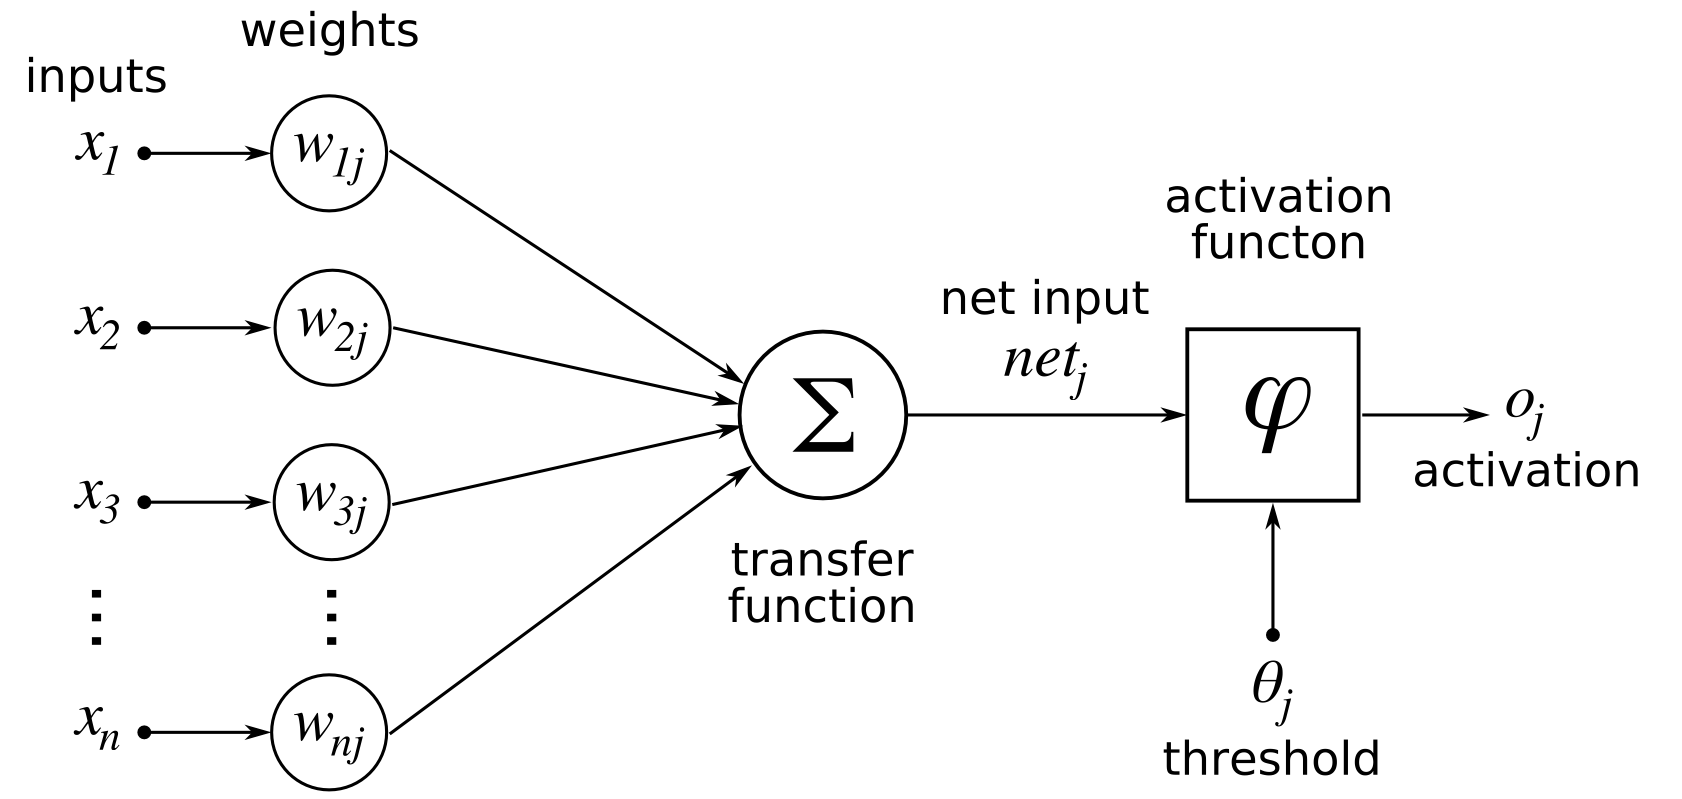
\includegraphics[width=.4\textwidth]{Neuron.png}
\caption{Artificial Neuron}
\label{fig:figure1}
\end{figure}

Knowing how artificial neurons works, we have to know how this neurons are organized inside the neural network. The neural network architecture is divided in, at least, two layers. One layer is called input layer, and the other one is called ouput layer. And, between this two layers, we can add one or more hidden layers. Of course we have to hae in mind that the bigger the numer of layers is, the more calculations and training complexity we have. We can se an example of a neural network with multiple layers in Figure \ref{fig:figure2}. Also, we have to think of the possibility of concatenate neural networks in order to solve more difficult problems or to build a better pipeline for the problem.

\begin{figure}[ht]
\centering
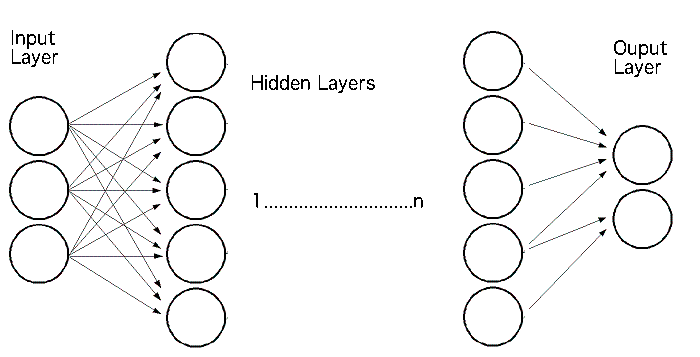
\includegraphics[width=.4\textwidth]{network.png}
\caption{Artificial Neuron}
\label{fig:figure2}
\end{figure}

Now, the matter is how a Neural Network can abstract the knowledge from the problems. The answer lies in the representation of the problem and, more specifically, in how we tune this model. So, firstly, we, as Deep Learning Engineers, must build a good representation of the problem for being understood by the computer. And lastly, we shloud tune the Neural Network in order to obtain the best results. This can be done by changing the number of layers, the way the layers are interconnected, the activation functions of the neurons, the restrictions of the supervised training, etc... Of course this procces of tunning is not easy, we can't be sure which configuration is going to work best and there is not a way to predict this.

Neural Networks have a lot of applications which the main ones are Character and Image recongnition, Image Compression, Stock Market Prediction and Some medicine applications such as cancer prediction.

\subsection{Unsupervised pretraining for Deep Architectures\cite{erhan2010does,bengio2007greedy}}
\label{sec:UnPre}
This section in the State of the Art is more important than It at first sight can seem. This is because, before 2006, Deep Learning was a field with not much progress and where the researchers obtained poor erros in the training and testing of the Deep Architectures, but the Unsupervised pretraining changed that fact and Deep Learning became into a field with a lot of future and applications.

The theory behind this is that, the large neural networks are difficult to train and it requires a large amount of time to get a good result but allway this result is not good enough. So, the main question that was disturbing the researchers was: Why do we get this poor results? The answer roots in the random initialization of the $\theta$ values for the layers and in the shape of the cost function.

The intuition behind this is that the cost function is not a simple one but it is a very coplex function with a really large amount of local minimums and when your algorithm starts to converge, it could be converging in a local minimum instead of converging in the global minimum or, at least, in a better one. In order to help the algorithm to converge faster, it is tipic to do a random inizialitation that situates the algorithm in a random place of the cost function and we could be near to a bad local minimum. So, before year 2006, Deep Learning because in the cost function for this kind of problems we have several local minimums and most of them are not good enough and, with the random initialization, we have a really great percentage to end into a not good enough local minimum. 

The solution was to do an unsupervised pretraining over the layers of the Deep Network to get a coherent initialization values for the $\theta$. But, why this solution works good? what is the meaning behing this unsupervised pretraining? The answer is still uncertain but are some papers that gives some ideas of this. The turth is that this papers give us an unswer to that question but thas answer is an intuition based on severals results obtained after the execute of various Deep algorithms.

The intuition behind this says that this supervised training acts as a regulization parameter that situates the initial state of the algorithm into a better place of the cost function, near a great local minimum. This means that, using a subset of the training examples without their label, the pretraining learns something about the inputs that gives us a better position in the cost function. Also, because we are really near to a good local minimum, we avoid the step to get closer to the local and, in result, we get a really faster convergence and, of course, we obtain a great results at the end.

The algorithms that are tipically used for the pretraining are the ones related to the neighborhood theory. For example the k-nearest algorith or others when you take the knwoledge that are various examples that should be neightbors to learn the values of $\theta$. The result is most than obvious, it is clearly proved that this process helps the algorithms to achieve better results and, also, you get a faster convergence which translates into less training time.

\subsection{Deep Neural Networks}
To add some extra information in the Neural Networks state of the art, I will use the book of Bengio \cite{bengio2009learning} to present some Neural Networks that are interesting to see. These Neural Networks are commonly used in Deep Architectures because they have particular characteristics that are going to be presented.

\subsubsection{Convolutional Neural Networks}
As we explainen in Section \ref{sec:UnPre}, the Deep Neural Networks were really difficult to train, but, among all of them, there is one that was the exception, it is the Convonutional Neural Network. The partiularity of this network is that is inspired in the structure of the visual system described and proposed by \cite{hubel1962receptive}.  The first attemps of this network were to apply the neurons with same parameters on patches of the previous layer obtaining a kind of transalational invariance. After that, another improvement to this model was the use of the error gradient obtaining a better performance. Now, for a quick recognition of objects, it is recognized that there is a consintentcy between the way the Convolutional Netorks process and the physiology of the visual system. Nowadays, the systems for pattern recogntinion that are based in Convolutional Neural Networks have the best performance. 

The peculiarity of Convolutional Neural Netowrks is that they have, normally, five or more layers and for the rest of the Deep Networks, the training with this amount of layers without an unsupervised pre-training become almost impossible to be done. Now, the question is Why this model has a better training than the others? The answer roots in the architecture.

The convolutional neural network of LeCun is divided by two types of layers, the first one is the convolutional layer and, the second one, the subsampling layer. All this layer have a topographic structure which means that the neurons have a coordenate associated that represents the area of the image where the neuron is receptive. We have that there are a rectangle patch that contains different numbers of neurons in each layer with the same weights for all of them.

One hypotesis explain the success of Convolutional Neural Networks because the neurons have a small fan-in which helps to the gradient to be propagated in all layers without becoming useless. But this explanation seems not to be good enough because the complexity of deep learning problems can not be performed that good only with the random sparse connectivity. The other hypotesis is based on the hierarchical local connectivity structure which is very strong an this kind of structure seems to be well suited for the vision tasks. Ther is also one interesting fact, a convulotional neural network with random initialization works better than a fully connected neural netowrk trained and worse than a optimized convolutional neural network. This fact seems to explain that convolutional neural networks are simply better suited for this kind of task thank to its structure.

\subsubsection{Boltzmann Machines}

Firstly, before the explanation of Boltzmann Machines, is worth to explain what an energy based model is, because Boltzman Macines are part of them.

The energy based models has set of variables of interest that have associated an energy value. The learning process in this models is done changing this value until it becomes desirable. The energy based models define a probability distribution using an energy function.

\begin{equation}
  p(x)=\frac{e^{-E(x)}}{Z}
\end{equation}

The $Z$ in the equation is a normalizing factor called partition function.

\begin{equation}
  Z=\displaystyle\sum_{x} e^{-E(x)}
\end{equation}

The learning process in energy based models can be done with stochastic gradient descent (Section \ref{sec:SGradient}), for example, but this has to be done on the empirical negative log likelihood of the training data set. 

Also, there are cases when the $x$ input is not seeing completely but we se a part of $x$ and we have a hidden part $h$, this particular case of energy based model is called Boltzmann Machine. This is done in special cases or when we want to have hidden parts in porpouse to increase the expressive power. Knowing this, the formula is different from the above one.
\begin{equation}
  P(x)=\displaystyle\sum_{h} P(x,h)=\displaystyle\sum_{h} \frac{e^{-E(x,h)}}{Z}
\end{equation}
Nota that now the sum is not over the $x$ input but over the $h$ hidden part. Now is tipic to introduce the formula of free energy to simplify this function into one easier.
\begin{equation}
  F(x)=- \log\displaystyle\sum_{h}{e^{-E(x,h)}}
\end{equation}
Then, now we have a new definition of the probability distibution after aplying the formula above to the formula of the probability distribution.
\begin{equation}
  P(x)=\frac{e^{-F(x)}}{Z}\quad \textrm{with}\quad Z= \displaystyle\sum_{h}{e^{-F(x)}}
\end{equation}

The Restricted Boltzmann Machines (RBMs) particularity is the they are more restric than Boltzmann machines having a structure without connections between the layer of the same type (visible-visible connection, hidden-hidden conection).

The energy function for RBMs is differetn from the energy function for BMs.
\begin{equation}
  E(u,v)= -b'v-c'v-h'Wv
\end{equation}
The $W$ represent the weights and $b'$ and $c'$ represents the offsets of the hidden and visible units. Now, the free energy formula change to:
\begin{equation}
  F(v)=-b'v - \displaystyle\sum_{i}\log\displaystyle\sum_{h_{i}}e^{h_{i}(c_{i}+W_{i}v)}
\end{equation}
And, nowing that the layers connections are independients we can write the next expression:
\begin{equation}
  p(h| v)=\prod_{i}p(h_{i}| v)\quad \textrm{and}\quad p(v| h)=\prod_{j}p(v_{i}|h)
\end{equation}
And, finally if we consider the commonly studied case of binary units we obtain another expressions. For the binary units case we have $v_{j},h_{i}\in\{0,1\}$ and the following expressions of the neuron activation function:
\begin{equation}
  p(h_{i}=1| v)= sigm(c_{i}+W_{i}v)\quad \textrm{and}\quad p(v_{j}=1| h)=sigm(b_{j}+W'_{j}h)
\end{equation}
And, the energy function with the free energy is:
\begin{equation}
  F(v)=-b'v - \displaystyle\sum_{i}\log(1+e^{(c_{i}+W_{i}v)})
\end{equation}
Finally, is worth to say that sampling in RBMs is useful for learning algorithms because with this we can obtain an estimator of the log-likelihood gradient which is used later to do the training in the update of the weights process.

\subsubsection{Deep Belief Networks}
Here is a section with a brief description of Deep Belief Networks.

Firstly, we have the architecture, where we have a RBM in the two deepest layers. So we have a neural network with a energy based layer with unsupervised training.
\begin{figure}[ht]
\centering
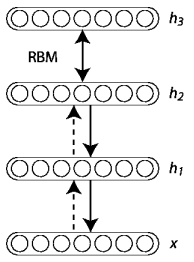
\includegraphics[width=.2\textwidth]{DBN.png}
\caption{Deep Belief Netork architecture}
\label{fig:figure3}
\end{figure}

Lastly, is worth to metion that the principle of greedy layer-wise unsupervised training\cite{bengio2007greedy} can be applied to the DBNs which we can described in 5 steps:
\begin{enumerate}
\item We have to train the first layer as it was a RBM that use the input $x=h^{(0)}$ on the visible layer.
\item We have now to use the first layer to obtain the input data for the second layer. We can use on of the two representations(mean activations $p(h^{(1)}=1|h^{(0)})$, samples $p(h^{(1)}|h^{(0)})$).
\item Train te first layer also as a visible layer of an RBM and taking the data from the step before as inputs.
\item Repeat the steps 2 and 3 until we have trained all of our layers.
\item Do a fine-tunning to the architecture. This tunning can be done with a normal supervised trainning used in the application of this work (Section \ref{sec:Architecture}) for example.
\end{enumerate}
That is the definition of DBN which is a composition of a RBM and a multilayer neural network.
\subsection{Other honorable mentions}
After the presentation of Boltzmann Machines and Neural Networks, I think is interesting to present another three algorithms that are also powerful and could be used to solve complex problems.

\subsubsection{Linear Regression}
Linear Regression is one of the mos used algorithms to predict a certain value or to classify from a serie of features that represent every input example. The intuition of this process is to draw a line through the examples which minimize the cost function. In order to understand this intuintion we can see the Figure \ref{fig:figure3}.

\begin{figure}[ht]
\centering
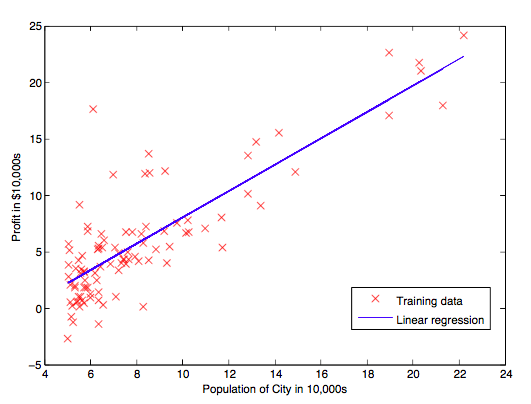
\includegraphics[width=.4\textwidth]{Regression.png}
\caption{Linear Regression}
\label{fig:figure3}
\end{figure}

So, in this algorithm we have two principal components. One is the cost function whose minimization is the objetive of Linear Regression. The second one is the hypotesis which is a linear function that represents the line to be drawn whose components are the $\theta$ value. 

Firstly, the cost functions is defined by the sum of the quadratic difference between the hypotesis and the objetive value of all training examples:

\begin{equation}
  J(\theta)=\frac{1}{2m} \displaystyle\sum_{i=1}^{m} (h_{\theta}(x^{(i)})-y^{(i)})^2
\end{equation}

Secondly, the hypotesis that is only a equation for a line but with the $\theta$ value that is going to change in the training in order to get the best fit for the data.

\begin{equation}
  h_{\theta}(x)=\theta^Tx=\theta_{0}+\theta_{1}x_{1}
\end{equation}

And this is Linear Regression algorithm which consist in draw the straight line through the training examples that minimize the cost function. Now, to obtain the best value $\theta$ for the problem, we have to use another algorithm and the most popular is Gradient Descent. And, in particular, we are going to present Batch Gradien Descent (see Section \ref{sec:Gradient}).

\subsubsection{Logistic Regression}
\label{sec:Logisic}
Logistic Regression has almost the same intuition as Linear Regression but in this case we are not trying to draw a straight line but a curve (See Figure \ref{fig:figure4}).
\begin{figure}[ht]
\centering
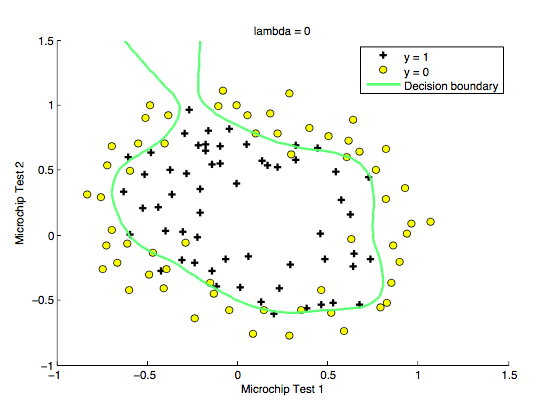
\includegraphics[width=.4\textwidth]{Logistic.png}
\caption{Logistic Regression}
\label{fig:figure4}
\end{figure}
Also, Logistic Regression algorithm has two components in its process to obtain the best curve to fit the data.

The first one is the cost function. The formula of the cost function for Logistic Regression seems harder than the formula for Linear Regression, but it is only the logarithmic function of the hypotesis or one minus the hypotesis dependind if the expected value is one or cero. So if the expected value is cero, then the cost function for that example is the logarithmic funtcion of one minus the hypotesis for that example, and, if the expected value is one, the cost functions is the logarithmic function of the hypotesis. The total cost function is the sum of the cost functions of all training examples. The formula is:
\begin{equation}
  J(\theta)=\frac{1}{m} \displaystyle\sum_{i=1}^{m} [-y^{(i)}\log(h_{\theta}(x^{(i)}))-(1-y^{(i)})\log(1 -h_{\theta}(x^{(i)}))]
\end{equation}
 The intuition for the formula is that, when you are trying to predict one, if the hypotesis is close to one the algorithmic function will return a number close to cero. And, if you are trying to predict cero, when the hyposetis is close to cero, we subtract a lower amount from the one value and we are requesting the logarithmic function value for a number close to one that is cero. So, when we are far from the expected value, the cost funciont is going to be higher.
 
 Now, the second component, is the hypotesis. Unlike in Linear Regression, in this algorithm we are trying to draw a curve that fits the data, so, the hypotesis is going to be a nonlinear function. In this case we are talking about the sigmoid function.
 
 \begin{equation}
  h_{\theta}(x)=g(\theta^Tx)=\frac{1}{1+e^{-\theta^Tx}}
\end{equation}

 And, like in Linear Regression, to calculate the $\theta$ value we have to perform an update for the $\theta$ using another algorithm. This algorithm can also be the Batch Gradient Descent (see Section \ref{sec:Gradient}).
\subsubsection{Batch Gradient Descent}
\label{sec:Gradient}
Batch Gradient Descent is an algorithm that determines the way we perform an update of the theta values. In every iteration of the training an uptdate is going to be performed. In Batch Gradien Descent we use all training examples to calculate the update needed to be performed. 

So, in each iteration of the algorithm, batch gradient descent is going to perform the update:

 \begin{equation}
 \theta_{j}:= \theta_{j} - \alpha \frac{1}{m} \displaystyle\sum_{i=1}^{m} (h_{\theta}(x^{(i)})-y^{(i)})x_{j}^{(i)}
\end{equation}

We have to know that this update is done simultaneously in $\theta_{j}$ for all $j$. With this update our $\theta$ parameter come closer to the optimal and, in result, our cost function $J(\theta)$ decrease achieving the lowest cost.

In order to increase the performance of the algorithm, it is common to use the gradient values. these gradients are calculated at the same time as the cost function increasing the overall performance.

\begin{equation}
 \frac{\partial J(\theta)}{\partial\theta_{j}}= \frac{1}{m} \displaystyle\sum_{i=1}^{m} (h_{\theta}(x^{(i)})-y^{(i)})x_{j}^{(i)}
\end{equation}

\subsubsection{Stochastic Gradient Descent}
\label{sec:SGradient}
This algorithm is another version of Gradient Descent, but for this particular algorithm, the updates are being done with other criteria. In the batch gradient descent, the information of the cost function of all examples is used to update the $\theta$. Because the updates are not doing with all examples, this algorithm is tipically used in problems with a large number of training examples in order to achieve a better performance. For this algorithm we have a specific cost function that it's normally used, but in our application we used other (see Section \ref{sec:Architecture}).

\begin{equation}
 cost(\theta,(x^{(i)},y^{(i)}))= \frac{1}{2}(h_{\theta}(x^{(i)})-y^{(i)})^2
\end{equation}

And, for the update, now we have an update with a different formula because we are using just one example.

 \begin{equation}
 \theta_{j}:= \theta_{j} - \alpha (h_{\theta}(x^{(i)})-y^{(i)})x_{j}^{(i)}
\end{equation}

As we can see, now we do not have a sum over all the examples, instead, we have the information of only one example. The new term in the formula is also a gradient of the cost function but with different parameters.

\begin{equation}
 \frac{\partial}{\partial\theta_{j}}cost(\theta,(x^{(i)},y^{(i)}))= (h_{\theta}(x^{(i)})-y^{(i)})x_{j}^{(i)}
\end{equation}

So, we have the next algorithm:
\begin{lstlisting}
from random import shuffle
#First shuffle of the examples
shuffle(data)
for i in range(numEpochs):
	for j in range(numTrainingExamples):
		Theta=Theta - alpha * gradient(cost(Theta,(x[j],y[j]))
\end{lstlisting}

The algorithm is to do an updatu for each examplo in each epoch. With this the cost function probaly, most in large umber of training examples, will have a lot of variations that will not be only a decrease variation but also a increase variation because when we have only the information of a single example its gradient could make the cost function have an increase in its total value.

To represent the cost function we have a formula that is represented as follows:
\begin{equation}
  J(\theta)=\frac{1}{m} \displaystyle\sum_{i=1}^{m}cost(\theta,(x^{(i)},y^{(i)}))
\end{equation}
There is at least another version of Gradien Descent, but since it is not used in this report and is no as basic as the Batch Gradient Descent it is not going to be presented in this paper.

\section{Model used in the application: Neural Networks}
Detailed presentation about Neural Networks. In this section I am going to writte the formulas and the meaning behind the basic Neural Networks. Also, the explanation of the vectorial implementation of the Neural Network is going to be explained because it is used in the application.

Firstly, we know that the minimum entity in a Neural Network is the neuron which has a set of weights depending on its inputs and an activation function. So we can say that, if we represent the activation function as $f$, the input as $x$ and the weights as $w$, the output of the nuerons is:
\begin{equation}
\textrm{output}(X,W)=f(\displaystyle\sum_{i}^{x}w^{(i)}x^{(i)})
\end{equation}
And, as we can see, we have that the input is a vector like $X=[x^{(0)},x^{(1)}...x^{(n)}$ and the weights is another vector of the same size like $W=[w^{(0)},w^{(1)}...w^{(n)}$. With this representation we can comprobate that we can do a vectorial implementation of this:
\begin{equation}
\textrm{output}(X,W)=f(W^{T}X)
\end{equation}
If we do that multiplication between $W^{T}$ and $X$ we have that now the $X$ is still a column vector and the $W$ is now a row vector, so, the result of the multiplication is going to be $W^{T}X = w^{(0)}x^{(0)}+w^{(1)}x^{(1)}+...+w^{(n)}x^{(n)}$ which is the same result as the non vectorial definition of the equation.

With this, we arrive at the representation of a layer. The representation of a layer is a group a of $m$ each with $n$ inputs that is the leng of the vector $X$ plus one because we have to add the bias. We saw that we can representate the weight of one neuron with a colum vector with $nX1$ dimension. So, we can representate the weights of one layer with a matrix with $nXm$ dimentions. If we have that $N$ represents the neurons and $L$ the current layer:
\begin{equation}
W_{(X)}^{(L)}= \theta_{(X)}^{(L)} = \bordermatrix{~ & N^{(1)} & N^{(2)} & \textrm{...} & N^{(m)} \cr X^{(1)} & w_{(1)}^{(1)} & w_{(2)}^{(1)}&\textrm{...}&w_{(1)}^{(m)} \cr X^{(2)} & w_{(2)}^{(1)} & w_{(2)}^{(2)}&\textrm{...}&w_{(2)}^{(m)} \cr \textrm{...} & \textrm{...} & \textrm{...} &\textrm{...}&. \cr X^{(n)}&w_{(n)}^{(1)}&w_{(n)}^{(2)}&\textrm{...}&w_{(n)}^{(m)}\cr}
\end{equation}
 So, now we have a matrix representing the layer with $m$ columns that is the number of neurons of that layer. So we still have the same formula to calculate the ouput of the layer. Because, when we transpose $W$ we have one row for each neuron, this implies that, when we do the multiplication betweent $W^T$ and $X$, we will obtain a colum vector with $mX1$ dimentions. This means that we are going to return the ouput of each layer in one row. If we apply the same theory when we had only one neuron, we will se that this matrix multiplication is exactly the same as what we do with the non vectorial implementation. But the vectorial implementation tends to have better performance.
 
 Therefore,we will have an iinput layer with the size of $X$ (represented with $n$) plus the bias, so the size is $n + 1$. This means that the first layer, with $m$ neurons, is going to be a matrix of $n+1Xm$ dimentions. Then, the next layer, with $m1$ neurons, is going to be a matrix of $m+1Xm1$ dimentions. And so on. Having that each output of each layer is goint to be the input to the next layer o the preicte value (see Figure \ref{fig:Multilayer}).
 
\begin{figure}[ht]
\centering
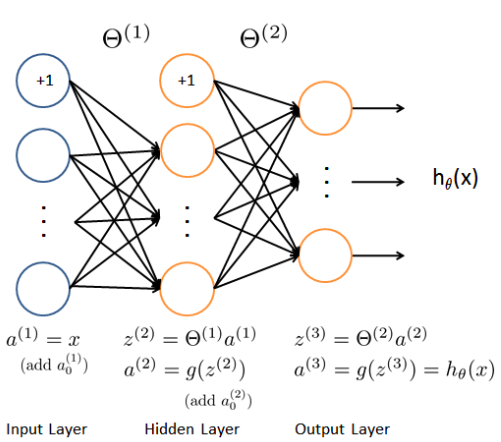
\includegraphics[width=.4\textwidth]{Multilayer.png}
\caption{Multilayer neural network}
\label{fig:Multilayer}
\end{figure}

Now, the $f$ activation function of the neurons, whe we are talking of a clasification problem, is normally the sigmoid function. This is because we are going to predict a probability betwee 0 and 1, both included, of one input to be of one class and the sigmoid function image has only that values. 

\begin{equation}
\textrm{sigmoid}(z)=g(z)=\frac{1}{1+e^{-z}}
\end{equation}

And its gradient cand be calculated with:

\begin{equation}
g'(z)=\frac{\partial}{\partial z}g(z)=g(z)(1-g(z))
\end{equation}

As we can see, the gradient is very easy to calculate which converts this activation function into a very convenient one.

In Neural Networks for classification we have that the cost function is the same as Logistic Regression (Section \ref{sec:Logistic}):
\begin{equation}
  J(\theta)=\frac{1}{m} \displaystyle\sum_{i=1}^{m} [-y^{(i)}\log(h_{\theta}(x^{(i)}))-(1-y^{(i)})\log(1 -h_{\theta}(x^{(i)}))]
\end{equation}
In order to control the learning rate and the process of learning exist a term knowing as regularization. In rest of the algorithms also exist this term but it was not described in this paper. But, in this section it is going to be described. In order to add the regularization we have a new variable $\lambda$ (lambda) which is the term to control the amoun of effect the regularization has over the cost function. And the regularization term is the sum of the squares of the $\theta$ values of every layer.
\begin{equation}
  \textrm{regularization}=\frac{\lambda}{2m} [\displaystyle\sum_{i=1}^{L}\displaystyle\sum_{j=1}^{N}\displaystyle\sum_{k=1}^{X} (\theta_{j,k}^{(i)})^2]
\end{equation}
In the equation above we have that $m$ is the number of input examples for the training. And that ther is not more than the process of sum all squares of the $\theta$ values from all layers. So, the regularized cost function is:
\begin{equation}
  J(\theta)=\frac{1}{m} \displaystyle\sum_{i=1}^{m} [-y^{(i)}\log(h_{\theta}(x^{(i)}))-(1-y^{(i)})\log(1 -h_{\theta}(x^{(i)}))] +\frac{\lambda}{2m} [\displaystyle\sum_{i=1}^{L}\displaystyle\sum_{j=1}^{N}\displaystyle\sum_{k=1}^{X} (\theta_{j,k}^{(i)})^2]
\end{equation}
In our application we did not use the regularized cost function, only the cost function. But this is not dificult to implement despite of to seem very dificult in the formula representation. The implementation in Theano for the cost function of our application (Section \ref{sec:Architecture}) would be:
\begin{lstlisting}
	cost_value=T.sum(-y*T.log(layer3)-(1-y)*T.log(1-layer3)) + T.sum(theta1**2) + T.sum(theta3**2) + T.sum(theta3**2)
\end{lstlisting}
The intuition behind the cost function is that in the $-\log$ function, the closer to the one you are, the less value you get. So, when we expect one, we do $1*-\log(h_{\theta}(x^{(i)}))$ obtaining less value the closer to cero we are. And, when we expect cero we do$1-0 * -\log(1-h_{\theta}(x^{(i)}))$, this means that when less is the value of the hypotesis, closer to one we are obtaining a less value from the $-\log$ function.

Afther this, to update the $\theta$ we can use one of the update algorithms described in this paper (Section \ref{sec:Gradient} and Section \ref{sec:SGradient}) or another one. Using all this knowledge the applitacion presented in this paper was made.
\section{Description of the application and its resuslts}

There are three main components to be described in this section. The first one is the architecture and tool used and developed for this application. The second one is the data used to train the model and to test it. And, the last one, is the results obtained while and afteher the training of the Neural Network.


\subsection{Architecture and tool}

Firstly, we choose the Theano tool because is one of the most popular tools and is for Python which is a very malleable and easy used. Also, in order to manage the arrays in a more convenient way we use Numpy for python.

\subsubsection{Theano\cite{2016arXiv160502688short}}
This tool for Python is one of the most populer ones to develop Deep Learning models. This is becaus Theano allows the user to run his code in the GPU and, also, it does a lot of compilations in C in order to achieve a better performance.

Theano also has a lot of functions and funtionalities that makes easy the job of implementing Deep Learning models. Theano allow us to work with expressions and representations of values and functions. So, if we want to work with Theano we have, at least, to know that this library works in other way. We have to define variables with types of Theano and used that variables to build functions. Also we have to know how shared variables works, because we used shared values for the weights.

The variables we used in our application are implementing as follows:
\begin{lstlisting}
    x = T.dvector('x') 
    y = T.dvector('y') 
    theta1 = theano.shared(np.array(np.random.rand(14,10), dtype=theano.config.floatX))
    theta2 = theano.shared(np.array(np.random.rand(11,5), dtype=theano.config.floatX))
    theta3 = theano.shared(np.array(np.random.rand(6,2), dtype=theano.config.floatX))
\end{lstlisting}
But we have to know that these variables are like the python's variables. These variables are a representation of what type of value is expected by Theano when we use the variables in the expression to define formulas, the cost function formula for example.
\begin{lstlisting}
	cost_value=T.sum(-y*T.log(layer3)-(1-y)*T.log(1-layer3))
\end{lstlisting}
This expression can be converted into a funtionc to be used in the future.
\begin{lstlisting}
    cost_function_test=theano.function(inputs=[x,y],outputs=[cost_value])
\end{lstlisting}
After implementing the function we can use it to get the cost function. We have to define the inputs using Theano variables. And the ouput can be a normal Python function or a Theano expression. Also, we can determine some updates to be done when the function is called.
\begin{lstlisting}
    cost_function=theano.function(inputs=[x,y],outputs=[cost_value],updates=[(theta1,gradient(cost_value,theta1,alpha)),(theta2,gradient(cost_value,theta2,alpha)),(theta3,gradient(cost_value,theta3,alpha))])    
\end{lstlisting}
If the update is done on variables that are not shared, then it has to be in the inputs. The ouputs are pairs with the variable to be updated and the value to update, can also be functions to calculate the new value. Now, we can use this function as a step of the train because we process one example and update the weights with the information of that example.

That was the basic information we used to implement our application with the Theano tool. For more information refer to the Theano Documentation.
\subsubsection{Architecture}
\label{sec:Architecture}
In order to manage this problem we decided to use the well known model of Neural Network. 

The Neural Network of our example has 3 layers.  The number of layers was decided for convention between the authors of the application and after testing the application with different numbers of layers and neurons. The best and most interesting results were obtained with the three layers we mentioned and with 10, 5 and 2 neurons respectively. The last layer, ouput layer, has 2 neurons, 1 neuron for each class.

The activation function for the neurons is the sigmoid function. This function was decided because for classification is one of the most populars ones. This is because the sigmoid function returns a value between 0 and 1, the values we want because we are predicting probabilities. So, in the ouput layer each layer is going to predict the probability of one example to be the class that the neuron represents.

For the training we decided to use the stochastic gradient descent algorithm. This algorithm is described in a previous section so to know more about it see the Section \ref{sec:SGradient}.

In the thery, for stochatic gradient descent we have the cost funtion described in its section, but in this case and using the theory of Neural Networks for classification we used the cost function described in the section of Neural Networks (Section \ref{sec:Neural Networks}).

And, the last detail to be mentioned is that we have a random values for the $\theta$ of the layers at the start of the application. This is noteworthy because one of the greatest advances in Deep Learning is the unsupervised pre-training\cite{erhan2010does,bengio2007greedy}. We decided this random initialization because we consider that the problem is not hard enough and the training examples are not enough to need this.

\subsection{Dataset Used: Heart Disease Data Set \cite{Lichman:2013}}
For this application we used a dataset with the data of the heart of some pacients and the information if they had a heart disease or not.This data was taken from four hospitals and it contains a total 76 features for each pacient, but the description said that only 14 features are used in the other works. Also, one of the dataset with 76 features is corrupted so we took the processed datasets with 14 features. \cite{heartDiseaseC,heartDiseaseZ,heartDiseaseH,heartDiseaseB}

The application take the data from the datasets and storage it to be treated. We do a shuffle of all training examples to mix the pacients of all hospitals. After that we prepare the data to be processed by the neural network.

Firstly, we split the data into two arrays. The first one is filled with the input examples with 13 features, and the second one is filled with the ouputs or the expected value with 1 feature. 

\begin{lstlisting}
shuffle(data) #Shuffle the data of all datasets
for i in data:
      inputs.append(i[:len(i)-1]) #Split the inputs
      outputs.append(i[len(i)-1]) #Split the expected outputs
\end{lstlisting}

The data in the ouputs array should be only 0 or 1 but some examples have the values 2 and 3 also, so we took all value greater than 0 as 1.

\begin{lstlisting}
for i in range(len(x)): #For values greater than 1 in the predicted value, we asume them as 1
        if x[i][len(x[i])-1] > 1:
            x[i][len(x[i])-1]=1
\end{lstlisting}

Now, the process is to convert the ouputs into an array because we are gonna have 2 neurons to predict two classes. The class heart disease ($[1,0]$) and the class no heart disease ($[0,1]$).

\begin{lstlisting}
    for i in outputs:                   #Converting the outputs to be predicted by 2 neurons
        if i==1:
            outputsF.append([1,0])
        else:
            outputsF.append([0,1])
\end{lstlisting}

Secondly, is to apply a mean normalization over tha features of the inputs examples. This process is done in order to have a better update of the $\theta$ and to reduce the difference between the features. Some features have a high values and other have only values of 0 and 1. The mean normalization is done with the next formula:

\begin{equation}
   \forall x \in X, \forall f \in, x^{(f)}= \frac{x^{(f)}-min(X^{(f)})}{max(X^{(f)})-min(X^{(f)})}
\end{equation}

We have that, for each input $x$ in the set of inputs $X$,  we do the process of normalization for each feature $f$ in the $x$ example. The normalization is done with the difference between the $f$ value in the example $x$ and the minimum value over all values of the feature $f$ in the set of inputs $X$ divided by the difference between the maximum value over all values of the feature $f$ in the set of inputs $X$ and the minumum described.

And lastly, the process is to divided the full dataset into two subdatasets. The first dataset is for the training process and it has the $70\%$ of all examples. The second dataset is for testing and it has the $30\%$ of all examples.
With that process we have the data ready to be used. To end this section a list of the features used and its descriptions is going to be presented.
 \begin{multicols}{2}
\begin{enumerate} 
	\item age: age in years 
	\item sex: sex (1 = male; 0 = female)
	\item cp: chest pain type 
	\begin{enumerate} 
		\item Value 1: typical angina 
		\item Value 2: atypical angina 
		\item Value 3: non-anginal pain 
		\item Value 4: asymptomatic 
	\end{enumerate}
	\item trestbps: resting blood pressure (in mm Hg on admission to the hospital) 
	\item chol: serum cholestoral in mg/dl 
	\item fbs: (fasting blood sugar > 120 mg/dl) (1 = true; 0 = false) 
	\item restecg: resting electrocardiographic results 
	\begin{enumerate} 
		\item Value 0: normal 
		\item Value 1: having ST-T wave abnormality (T wave inversions and/or ST elevation or depression of > 0.05 mV)  
		\item Value 2: showing probable or definite left ventricular hypertrophy by Estes' criteria 
	\end{enumerate}
	\item thalach: maximum heart rate achieved 
	\item exang: exercise induced angina (1 = yes; 0 = no)
	\item oldpeak = ST depression induced by exercise relative to rest 
	\item slope: the slope of the peak exercise ST segment 
	\begin{enumerate} 
		\item Value 1: upsloping 
		\item Value 2: flat   
		\item Value 3: downsloping 
	\end{enumerate}
	\item ca: number of major vessels (0-3) colored by flourosopy
	\item thal: 3 = normal; 6 = fixed defect; 7 = reversable defect
	\item num: diagnosis of heart disease (angiographic disease status)
\end{enumerate}
\end{multicols}
\subsection{Results}
After many executions of the application we had differents results. I think that this contrast in the results that is because we do a random inizalitation of the values of $\theta$. When we this inicialization we could have a good values for $\theta$ and get a better convergence of the cost function, but when the random values are bad we do not get a very good convergence of the cost function and, in result, we obtain a model with a less success rate. The best hit rate we obtained was the $83\%$ of hits.

Also we studied the progress of the cost function for the test inputs and for the training inputs in every epoch. We could see different situations, also depending on good or bad values for $\theta$. One situation is when we do not get good values and the  test cost is not the good that it could be. Other situation is when the values are too goods and the training produces a overfitting obtaining a drecreasing cost for training and increasing cost for test. And the las one is when we get good enough values to get a good training with a normal behavior for the costs.

In the graphs (Figure \ref{Fig:Data1} and Figure \ref{Fig:Data2}) we are going to be able to se some results obtained during the training. The blue dots represent the test cost function and the red dots the training cost function. And the green dots represent the hits and the red dots the misses in the other graphs.
\begin{figure}[!htb]
   \begin{minipage}{0.48\textwidth}
     \centering
     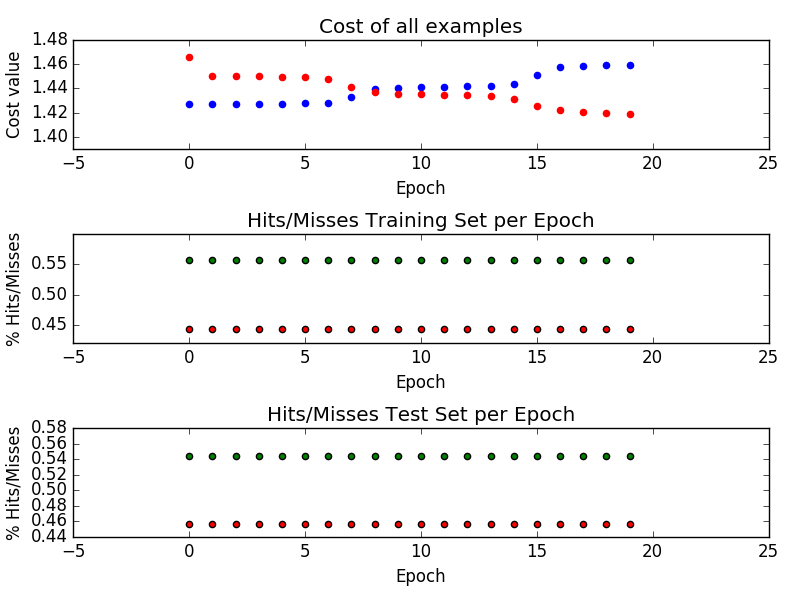
\includegraphics[width=.9\linewidth]{Plot_29_01_2017_22_26.png}
     \caption{Training with overfit}\label{Fig:Data1}
   \end{minipage}\hfill
   \begin {minipage}{0.48\textwidth}
     \centering
     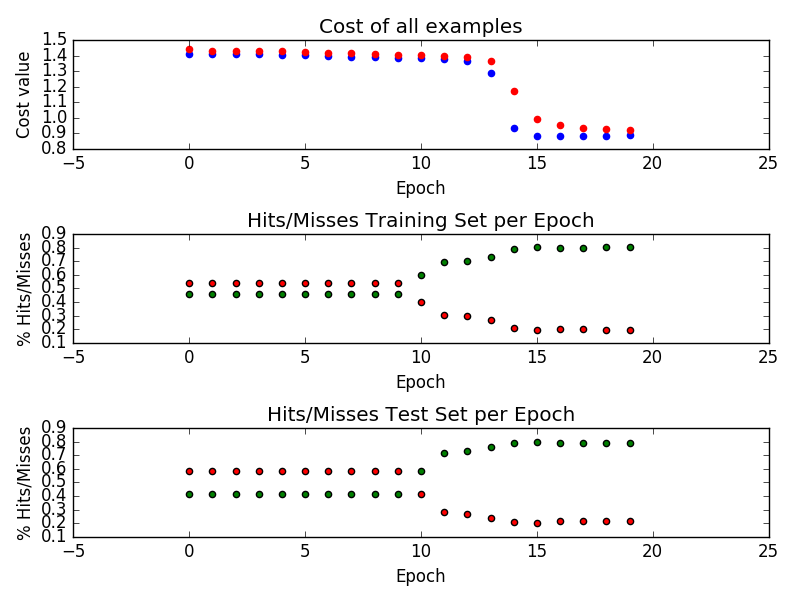
\includegraphics[width=.9\linewidth]{Plot_30_01_2017_03_42.png}
     \caption{Training with nice fit}\label{Fig:Data2}
   \end{minipage}
\end{figure}
\section{Conclusion}
In conclusion, I was able to see the complex task of work in Deep Learning. Also, I was able to understand that the models and architecures for this field are very difficult and the maths behind them are also difficult. If one person want to do improves in these architectures and do researching about this topic, he should have a minimum level of calculus.

Furthermore, I was able to see the great future of this field because these architectures are able to perform a really complex tasks. And with the continuous improvement of these architectures the peroformanes is going to get better, so this field could one day perform even more complex tasks and become a necessary technology for our lives.

Lastly, I have to admit that I really enjoyed the process of learning and implementing this architectures using real data, so I am going to continue studying and developing more dificult tasks and architectures.
\bibliography{sbc-template}
\bibliographystyle{plain}

\end{document}
